% !TEX TS-program = pdflatex
% !TEX encoding = UTF-8 Unicode

\documentclass{beamer}
% for handouts: \documentclass[handout]{beamer}

%\setbeamertemplate{background canvas}[vertical shading][bottom=white,top=structure.fg!25]
% or whatever

\usetheme[compress]{Amsterdam}
%\setbeamertemplate{headline}{}
%\setbeamertemplate{footline}{}
%\setbeamersize{text margin left=0.5cm}
  
\usepackage[english]{babel}
\usepackage{listings}
\usepackage{geometry}
\usepackage{hyperref}

\usepackage{color}
\usepackage[T1]{fontenc}
\usepackage[utf8]{inputenc}
\usepackage{lmodern}

\usepackage{multicol}
\lstset{
basicstyle=\scriptsize\ttfamily,
columns=flexible,
breaklines=true,
numbers=left,
%stepsize=1,
numberstyle=\tiny,
backgroundcolor=\color[rgb]{0.85,0.90,1}
}


\begin{document}

\title[Big Data and Automated Content Analysis]{\textbf{Big Data and Automated Content Analysis\\ Part I+II} \\ Week 9 -- Wednesday \\ »Supervised Machine Learning I«}
\author[Damian Trilling]{Damian Trilling \\ ~ \\ \footnotesize{d.c.trilling@uva.nl \\@damian0604} \\ \url{www.damiantrilling.net}}
\date{10 April 2019}
\institute[UvA]{Afdeling Communicatiewetenschap \\Universiteit van Amsterdam}


\begin{frame}{}
\titlepage
\end{frame}

\begin{frame}{Today}
\tableofcontents
\end{frame}




\section[Recap]{Recap: Types of Automated Content Analysis}
\begin{frame}{}
Recap: Types of Automated Content Analysis
\end{frame}
\subsection*{Top-down vs. bottom-up}


%{\setbeamercolor{background canvas}{bg=black}
\begin{frame}[plain]
\makebox[\linewidth]{
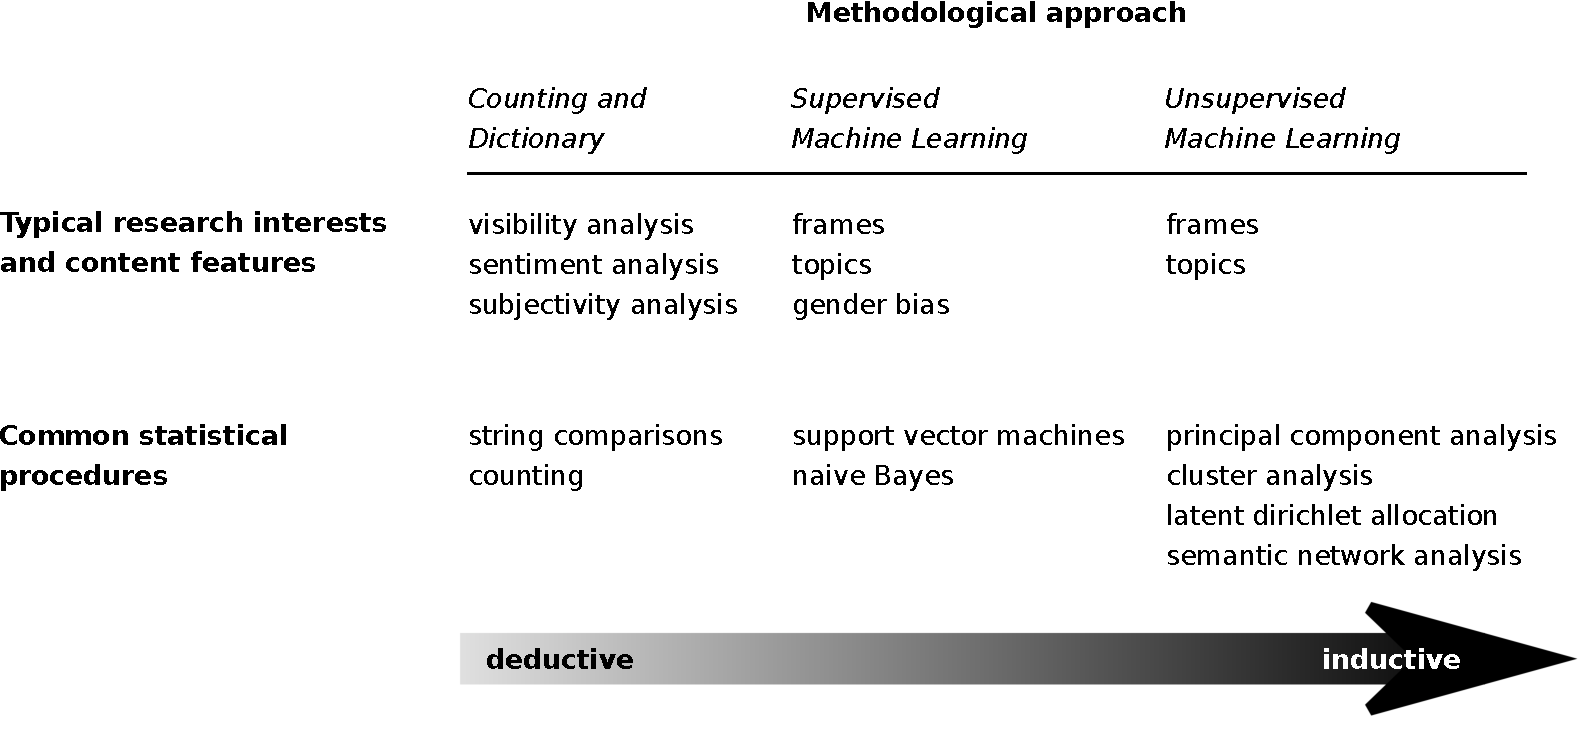
\includegraphics[width=\paperwidth,height=\paperheight,keepaspectratio]{../../pictures/boumanstrilling2016}}
\end{frame}
%}




\begin{frame}{Some terminology }
	\begin{columns}[t]
		\column{.5\textwidth}
		
		\begin{block}<1-4>{Supervised machine learning}
			You have a dataset with both predictor and outcome (independent and dependent variables; features and labels) --- a \emph{labeled} dataset.
			\onslide<2>{
				\footnotesize{Think of regression: You measured \texttt{x1}, \texttt{x2}, \texttt{x3} and you want to predict \texttt{y}, which you also measured}}
		\end{block}
		
		\column{.5\textwidth}
		
		\begin{block}<3->{Unsupervised machine learning}
			You have no labels. \onslide<4>{(\footnotesize{You did not measure \texttt{y})}}\\
			\onslide<5>{\textbf{Again, you already know some techniques to find out how \texttt{x1}, \texttt{x2},\ldots \texttt{x\_i} co-occur from other courses:} \begin{itemize}
					\item Principal Component Analysis (PCA)
					\item Cluster analysis
					\item \ldots
				\end{itemize}
			}
		\end{block}
		
	\end{columns}
	
\end{frame}






\section{Supervised Machine Learning}






\subsection{You have done it before!}
\begin{frame}{You have done it before!}
\begin{block}{Regression}<2->
	\begin{enumerate}
		\item<3-> Based on your data, you estimate some regression equation 	$y_i = \alpha + \beta_1 x_{i1} + \cdots + \beta_p x_{ip} + \varepsilon_i$
		\item<4-> Even if you have some \emph{new unseen data}, you can estimate your expected outcome $\hat{y}$!
		\item<5-> Example: You estimated a regression equation where $y$ is newspaper reading in days/week: $y = -.8 + .4 \times man + .08 \times age$
		\item<6-> You could now calculate $\hat{y}$ for a man of 20 years and a woman of 40 years -- \emph{even if no such person exists in your dataset}: \\
		$\hat{y}_{man20} = -.8 + .4 \times 1 + .08 \times 20 = 1.2$ \\
		$\hat{y}_{woman40} = -.8 + .4 \times 0 + .08 \times 40 = 2.4$
	\end{enumerate}
\end{block}	

\end{frame}


\begin{frame}{}
	\huge{This is\\ Supervised Machine Learning!}
\end{frame}

\begin{frame}{\ldots but\ldots}
	\begin{itemize}
		\item<1-> We will only use \emph{half} {\tiny{(or another fraction)}} of our data to estimate the model, so that we can use the other half to check if our predictions match the manual coding (``labeled data'',``annotated data'' in SML-lingo)
		\begin{itemize}
			\item<2->e.g., 2000 labeled cases, 1000 for training, 1000 for testing --- if successful, run on 100,000 unlabeled cases
		\end{itemize}
		\item<3-> We use many more independent variables (``features'')
		\item<4-> Typically, IVs are word frequencies (often weighted, e.g. tf$\times$idf) ($\Rightarrow$BOW-representation)
	\end{itemize}
\end{frame}


\subsection{Applications}

\begin{frame}{Applications}
\begin{block}<2->{In other fields}
\emph{A lot} of different applications
\begin{itemize}
\item from recognizing hand-written characters to recommendation systems
\end{itemize}
\end{block}

\begin{block}<3>{In our field}
It starts to get popular to measure latent variables
\begin{itemize}
\item frames
\item topics
\end{itemize}
\end{block}
\end{frame}



\begin{frame}{SML to code frames and topics}
\begin{block}{Some work by Burscher and colleagues}
\begin{itemize}
\item Humans can code generic frames (human-interest, economic, \ldots)
\item Humans can code topics from a pre-defined list 
\item<2->\textbf{But it is very hard to formulate an explicit rule} \\(as in: code as 'Human Interest' if regular expression R is matched)
\end{itemize}
\onslide<3>$\Rightarrow$ This is where you need supervised machine learning!
\end{block}
\tiny{Burscher, B., Odijk, D., Vliegenthart, R., De Rijke, M., \& De Vreese, C. H. (2014). Teaching the computer to code frames in news: Comparing two supervised machine learning approaches to frame analysis. \emph{Communication Methods and Measures, 8}(3), 190–206. doi:10.1080/19312458.2014.937527
\\
Burscher, B., Vliegenthart, R., \& De Vreese, C. H. (2015). Using supervised machine learning to code policy issues: Can classifiers generalize across contexts? \emph{Annals of the American Academy of Political and Social Science, 659}(1), 122–131.
}

\end{frame}





{\setbeamercolor{background canvas}{bg=black}
\begin{frame}[plain]
\makebox[\linewidth]{
\includegraphics[width=\paperwidth,height=\paperheight,keepaspectratio]{../../pictures/burscher2014}}
\end{frame}

\begin{frame}[plain]
\makebox[\linewidth]{
\includegraphics[width=\paperwidth,height=\paperheight,keepaspectratio]{../../pictures/burscher2015-a}}
\end{frame}

\begin{frame}[plain]
\makebox[\linewidth]{
\includegraphics[width=\paperwidth,height=\paperheight,keepaspectratio]{../../pictures/burscher2015-b}}
\end{frame}
}

\begin{frame}[plain]
\begin{columns}[]
\column{.5\textwidth}

{\tiny{http://commons.wikimedia.org/wiki/File:Precisionrecall.svg}}
\makebox[\linewidth]{
\includegraphics[width=\paperwidth,height=\paperheight,keepaspectratio]{../../pictures/precisionrecall.png}}

\column{.5\textwidth}
\begin{block}{Some measures of accuracy}
\begin{itemize}
\item Recall
\item Precision
\item $\text{F1}=2\cdot \frac{\text{precision}\cdot \text{recall}}{\text{precision}+\text{recall}}$
\item AUC (Area under curve) $[0,1]$, $0.5=$ random guessing
\end{itemize}
\end{block}


\end{columns}

\end{frame}





\begin{frame}{What does this mean for our research?}
\begin{block}<2>{It we have 2,000 documents with manually coded frames and topics\ldots}
\begin{itemize}
\item we can use them to train a SML classifier
\item which can code an unlimited number of new documents
\item with an acceptable accuracy
\end{itemize}
\end{block}
\onslide<2>{
\tiny{Some easier tasks even need only 500 training documents, see Hopkins, D. J., \& King, G. (2010). A method of automated nonparametric content analysis for social science. \emph{American Journal of Political Science, 54}(1), 229–247.}} 
\end{frame}



\subsection{An implementation}

\begin{frame}[fragile]{An implementation}
Let's say we have a list of tuples with movie reviews and their rating:
\begin{lstlisting}
reviews=[("This is a great movie",1),("Bad movie",-1), ... ...]
\end{lstlisting}
And a second list with an identical structure:
\begin{lstlisting}
test=[("Not that good",-1),("Nice film",1), ... ...]
\end{lstlisting}
Both are drawn from the same population, it is pure chance whether a specific review is on the one list or the other.\\
\tiny{Based on an example from \url{http://blog.dataquest.io/blog/naive-bayes-movies/}}
\end{frame}


\begin{frame}[fragile]{Training a A Naïve Bayes Classifier}
\begin{lstlisting}
from sklearn.naive_bayes import MultinomialNB
from sklearn.feature_extraction.text import CountVectorizer
from sklearn import metrics
 
# This is just an efficient way of computing word counts
vectorizer = CountVectorizer(stop_words='english')
train_features = vectorizer.fit_transform([r[0] for r in reviews])
test_features = vectorizer.transform([r[0] for r in test])
 
# Fit a naive bayes model to the training data.
nb = MultinomialNB()
nb.fit(train_features, [r[1] for r in reviews])
 
# Now we can use the model to predict classifications for our test features.
predictions = nb.predict(test_features)
actual=[r[1] for r in test]

print("Precision: {0}".format(metrics.precision_score(actual, predictions, pos_label=1, labels = [-1,1])))
print("Recall: {0}".format(metrics.recall_score(actual, predictions, pos_label=1, labels = [-1,1])))
\end{lstlisting}
\end{frame}
%
%\begin{frame}{TODO}
%TODO\\
%andere vectorizer (TFIDF)\\
%verschillen classifiers\\
%andere output (metrics summary)
%\\
%waarom is dit hier een MULTINOMIAL NB
%\\
%scikit-learn installeren\\ 
%opdracht bedenken: classifiers vergelijken
%\end{frame}


\begin{frame}{And it works!}
Using 50,000 IMDB movies that are classified as either negative or positive,
\begin{itemize}
\item I created a list with 25,000 training tuples and another one with 25,000 test tuples and
\item trained a classifier
\item that achieved an AUC of .82.
\end{itemize}
~\\
\tiny{Dataset obtained from \url{http://ai.stanford.edu/~amaas/data/sentiment}, Maas, A.L., Daly, R.E., Pham, P.T., Huang, D., Ng, A.Y., \& Potts, C. (2011). Learning word vectors for sentiment analysis. \emph{49th Annual Meeting of the Association for Computational Linguistics (ACL 2011)}
}

\end{frame}

\begin{frame}[fragile]{Playing around with new data}
\begin{lstlisting}
newdata=vectorizer.transform(["What a crappy movie! It sucks!", "This is awsome. I liked this movie a lot, fantastic actors","I would not recomment it to anyone.", "Enjoyed it a lot"])
predictions = nb.predict(newdata)
print(predictions)
\end{lstlisting}
This returns, as you would expect and hope:
\begin{lstlisting} 
[-1  1 -1  1]
\end{lstlisting}


\end{frame}




\begin{frame}{But we can do even better}
We can use different vectorizers and different classifiers.
\end{frame}



\section{Vectorizers}

\begin{frame}[plain]
\textbf{Vectorizers}
\end{frame}

\begin{frame}{Different vectorizers}
\begin{enumerate}[<+->]
	\item CountVectorizer (=simple word counts)
	\item TfidfVectorizer (word counts (``term frequency'') weighted by number of documents in which the word occurs at all (``inverse document frequency''))
\end{enumerate}

\pause
$$tfidf_{t,d} = tf_{t,d} \cdot idf_{t}$$

There are different ways to weigh the idf score. A common one is taking the logarithm:

$$idf_{t} = \log \frac{N}{n_t}$$

where $N$ is the total number of documents and $n_t$ is the number of documents containing term $t$
\end{frame}

\begin{frame}{Different vectorizer options}
\begin{itemize}
	\item Preprocessing (e.g., stopword removal)
	\item Remove words below a specific threshold (``occurring in less than $n=5$ documents'') $\Rightarrow$ spelling mistakes etc.
	\item Remove words above a specific threshold (``occuring in more than 50\% of all documents) $\Rightarrow$ de-facto stopwords
	\item Not only to improve prediction, but also performance (can reduce number of features by a huge amount)
\end{itemize}
\end{frame}








\section{Different models}


\begin{frame}[plain]
\textbf{Models (Classifiers)}

\vspace{1cm}

\footnotesize{(When we want to predict a binary outcome, we often refer to this as a \emph{classification problem}, while we often call predicting a continous outcome a \emph{regression problem}.)}
\end{frame}

\begin{frame}{Different classifiers}
	\begin{itemize}
		\item Naïve Bayes
		\item Logistic Regression
		\item Support Vector Machine (SVM)
		\item \ldots
	\end{itemize}
Typical approach: Find out which setup performs best (see example source code in the book).
\end{frame}



\begin{frame}{Naïve Bayes}
\begin{block}{Bayes' theorem}
$$ P(A \mid B) = \frac{P(B \mid A) \times P(A)}{P(B)} $$
\end{block}

\pause
\textcolor{red}{A = Text is about sports\\
B = Text contains ``a very good game''}
\pause
Furthermore, we simply multiply the propabilities for the features:
\textcolor{red}{$$P(B) = P(a\, very\, close\, game) = P(a) \times P(very) \times P(close) \times P(game)$$}
We can fill in all values by counting how many articles are about sports, and how often the words occur in these texts.
\vspace{0.3cm}

\footnotesize{
(Fully elaborated example on \url{https://monkeylearn.com/blog/practical-explanation-naive-bayes-classifier/})}

\end{frame}


\begin{frame}{Naïve Bayes}
\begin{itemize}[<+->]
	\item It's ``naïve'' because the features are treated as completely independent ($\neq$ ``controlling'' in regression analysis)
	\item It's fast and easy
	\item It's a good \emph{baseline} for binary classification problems
\end{itemize}
\end{frame}


\begin{frame}{Logistic Regression}
\begin{block}{Probability of a binary outcome in a regression model}
$$p = \frac{1}{1 + e^{-(\beta_0 + \beta_1 x_1 + \beta_2 x_2 + \ldots + \beta_n x_n)}}$$
\end{block}
Just like in OLS regression, we have an intercept and regression coefficients. 

We use a threshold (default: 0.5) and above, we assign the positive label (`good movie'), below, the negative label (`bad movie').

\end{frame}

\begin{frame}{Logistic Regression}
\begin{itemize}[<+->]
\item The features are \emph{not} independent.
\item Computationally more expensive than Naïve Bayes
\item We can get probabilities instead of just a label
\item That allows us to say how sure we are for a specific case
\item \ldots or to change the threshold to change our precision/recall-tradeoff
\end{itemize}
\end{frame}



\begin{frame}{Support Vector Machines}

\begin{columns}
	\column{.5\linewidth}
	\begin{itemize}
	\item	Idea: Find a hyperplane that best seperates your cases
	\item Can be linear, but does not have to be (depends on the so-called kernel you choose)
	\item Very popular 
\end{itemize}
	
	\column{.5\linewidth}	
		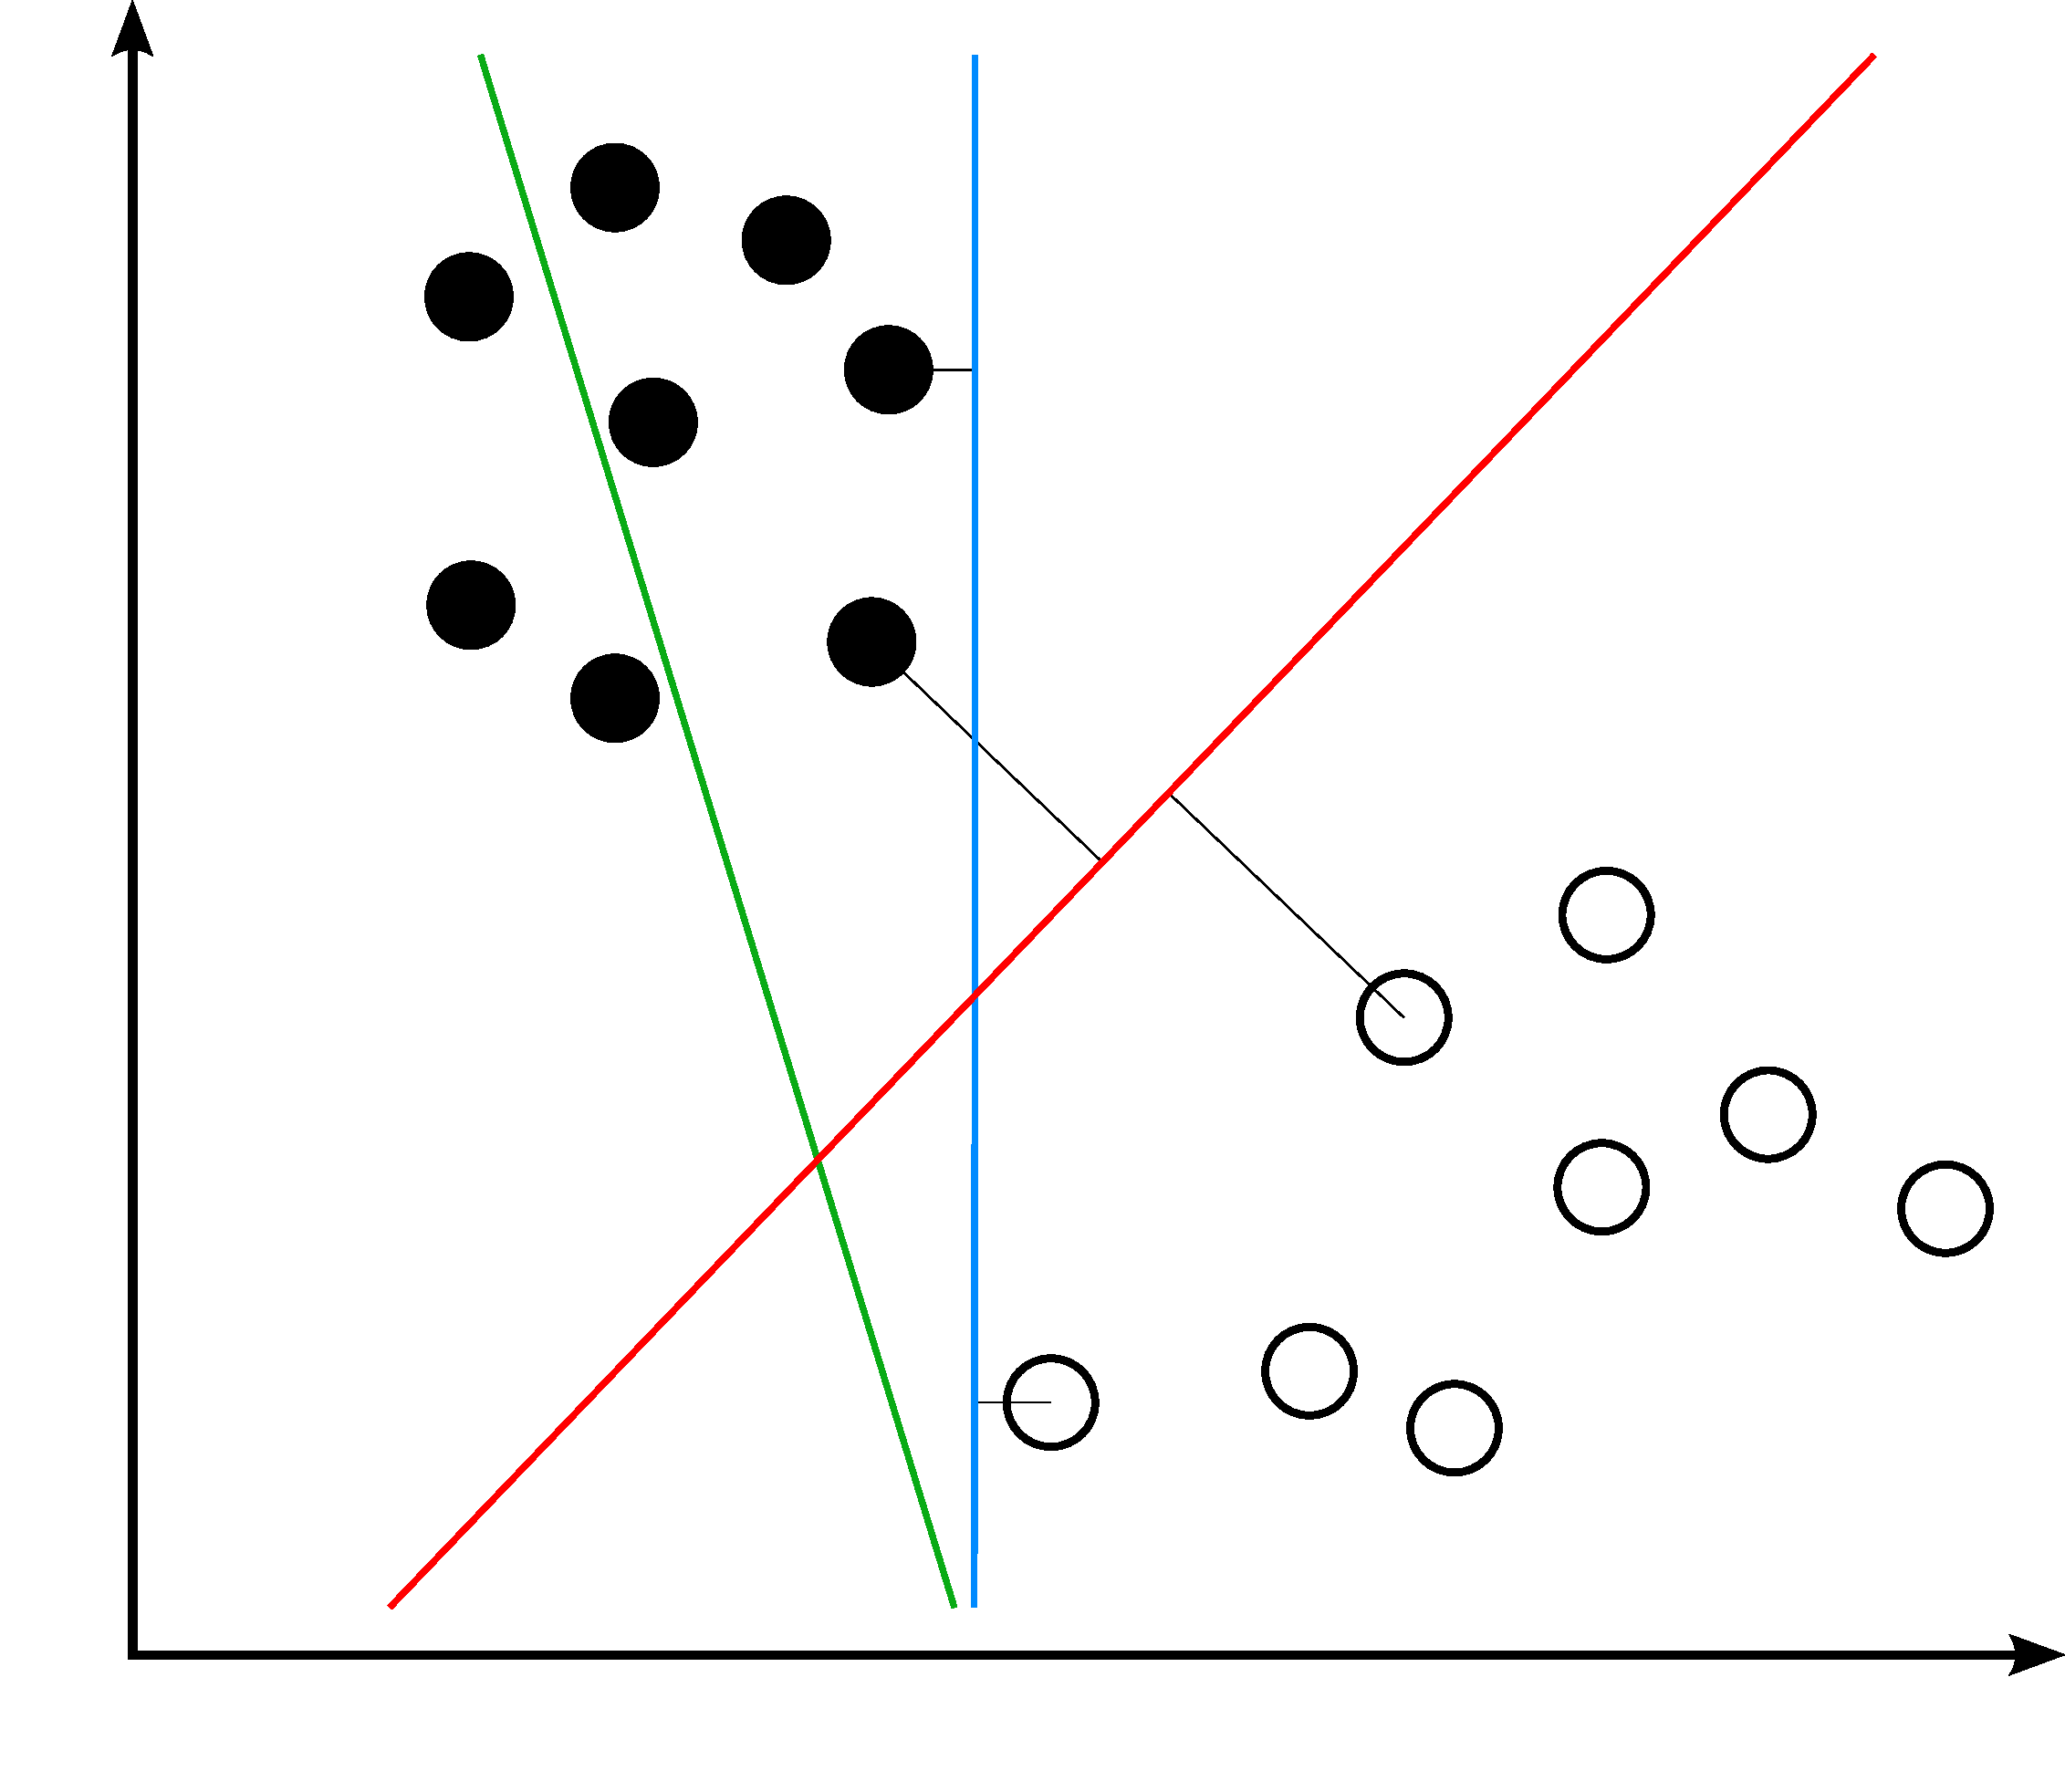
\includegraphics[width=.8\linewidth,height=.5\paperheight,keepaspectratio]{../../pictures/svm}
	\tiny{\url{https://upload.wikimedia.org/wikipedia/commons/b/b5/Svm\_separating\_hyperplanes\_\%28SVG\%29.svg}}
	
	\end{columns}
\vfill
\footnotesize{(Further reading: \url{https://monkeylearn.com/blog/introduction-to-support-vector-machines-svm/)}}
\end{frame}



\begin{frame}{Decision Trees and Random Forests}

\begin{columns}
	\column{.5\linewidth}
	\begin{itemize}[<+->]
		\item Model problem as a series of decisions (e.g., if cloudy then \ldots if temperature > 30 degrees then \ldots)
		\item Order and cutoff-points are determined by an algorithm
		\item Big advantage: Model non-linear relationships
		\item And: They are easy to interpret (!) (``white box'')
	\end{itemize}
	
	\column{.5\linewidth}	
	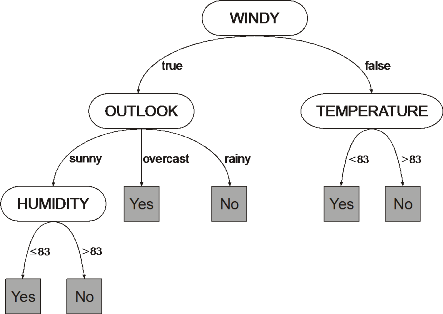
\includegraphics[width=.8\linewidth,height=.5\paperheight,keepaspectratio]{../../pictures/decisiontree}
	\tiny{\url{https://upload.wikimedia.org/wikipedia/en/4/4f/GEP\_decision\_tree\_with\_numeric\_and\_nominal\_attributes.png}}
	
\end{columns}

\end{frame}



\begin{frame}{Decision Trees and Random Forests}

\begin{block}{Disadvantages of decision trees}
\begin{itemize}
	\item comparatively inaccurate
	\item once you are in the wrong branch, you cannot go `back up'
	\item prone to overfitting (e.g., outlier in training data may lead to completely different outcome)
\end{itemize}
\end{block}

\pause

Therfore, nowadays people use \emph{random forests}: Random forests \emph{combine} the predictions of \emph{multiple} trees

$\Rightarrow$ might be a good choice for your non-linear classification problem

\end{frame}

\begin{frame}
\large{\url{https://scikit-learn.org/stable/supervised_learning.html}}
\end{frame}




\section{Next meetings}
\begin{frame}{Next meetings}
\begin{block}{Friday}
We'll write a supervised machine learning classifier (Chapter 10)
\end{block}

\begin{block}{Next Wednesday: Supervised machine leraning 2}
Creating the best model using Cross Validation, different thresholds, ROC curves, different feature sets, \ldots
\end{block}



\end{frame}




\end{document}

